% !TeX spellcheck = ru_RU
\documentclass[14pt, a4paper, fleqn]{extreport}

\usepackage{amsthm,amsfonts,amsmath,amssymb,amscd}
\usepackage[T2A]{fontenc}                         
\usepackage[utf8]{inputenc}                      
\usepackage[english, russian]{babel}
\usepackage{graphicx}
\usepackage{indentfirst}
\usepackage{cite} 
\usepackage{psfrag}
\usepackage{subcaption}
\usepackage{esint}
\usepackage[top=2cm,bottom=2cm,left=2.5cm,right=1cm]{geometry}

\linespread{1.3} 

\usepackage{ucs}
\usepackage{lineno}
\usepackage{graphicx}
\usepackage{float}
\usepackage{hyperref}

\begin{document}
	
	\newcommand{\round}[1]{\stackrel{o}{#1}}
	\newcommand{\grad}{\text{grad }}
	\renewcommand{\div}{\text{div }}
	\newcommand{\rot}{\text{rot }}
	\newcommand{\hess}{\text{hess }}
	\newcommand{\laplace}{\mathop{}\!\mathbin\bigtriangleup}
		
	\begin{titlepage}
	\begin{center}
		
\includegraphics[width=8cm, height=4cm]{MSU}
	\end{center}
	\begin{center}
			Московский государственный университет имени М.В. Ломоносова\\
			\vspace{0.1 cm}
			Факультет вычислительной математики и кибернетики\\
			\vspace{0.1 cm}
			Кафедра вычислительных методов
			
			\vspace{3cm}
			{\Large Бутаков Олег Борисович }\\
			\vspace{1cm}
			
			{\bf\LARGE <<to be filled by the OEM>>}\\ \vspace{2cm}
			КУРСОВАЯ РАБОТА
	\end{center}
	\vspace{2cm}
	\begin{flushright}
		{\bf Научный руководитель:}\\
		     д.ф-м.н., профессор \\
			 С.И. Мухин
	\end{flushright}		
	\vspace{4.5cm}
	\centerline {Москва, 2019}
	\end{titlepage}
	
	\tableofcontents
	\clearpage
	
	%%%%%%%%%%%%%%%%%%%%%%%%%%%%%%%%%%%%%%%%%%%%%%%%%%%%%%%%%%%%%%%%%%%%%%%%%%%%%%
	%%%%%%%%%%%%%%%%%%%%%%%%%%%%%%%%%%%%%%%%%%%%%%%%%%%%%%%%%%%%%%%%%%%%%%%%%%%%%%
	\chapter*{Введение}
	%%%%%%%%%%%%%%%%%%%%%%%%%%%%%%%%%%%%%%%%%%%%%%%%%%%%%%%%%%%%%%%%%%%%%%%%%%%%%%
	%%%%%%%%%%%%%%%%%%%%%%%%%%%%%%%%%%%%%%%%%%%%%%%%%%%%%%%%%%%%%%%%%%%%%%%%%%%%%%
	\addcontentsline{toc}{chapter}{Введение} 
		
	В данной работе рассматриваются основные свойства 
	системы уравнений магнитной гидродинамики,
	а также наиболее популярные на сегодняшний день способы её численного решения:
	такие как схемы Годуновсткого типа и разрывный метод Галеркина.
		
	%%%%%%%%%%%%%%%%%%%%%%%%%%%%%%%%%%%%%%%%%%%%%%%%%%%%%%%%%%%%%%%%%%%%%%%%%%%%%%
	%%%%%%%%%%%%%%%%%%%%%%%%%%%%%%%%%%%%%%%%%%%%%%%%%%%%%%%%%%%%%%%%%%%%%%%%%%%%%%
	\chapter{Система уравнений магнитной гидродинамики.}
	%%%%%%%%%%%%%%%%%%%%%%%%%%%%%%%%%%%%%%%%%%%%%%%%%%%%%%%%%%%%%%%%%%%%%%%%%%%%%%
	%%%%%%%%%%%%%%%%%%%%%%%%%%%%%%%%%%%%%%%%%%%%%%%%%%%%%%%%%%%%%%%%%%%%%%%%%%%%%%
	
	%%%%%%%%%%%%%%%%%%%%%%%%%%%%%%%%%%%%%%%%%%%%%%%%%%%%%%%%%%%%%%%%%%%%%%%%%%%%%%
	\section{Система уравнений магнитной \\
		     гидродинамики.}
	%%%%%%%%%%%%%%%%%%%%%%%%%%%%%%%%%%%%%%%%%%%%%%%%%%%%%%%%%%%%%%%%%%%%%%%%%%%%%%
	
	Система уравнений магнитной гидродинамики (\ref{mhd_system}) описывает
	течение вязкой проводящей жидкости или газа.
	
	\begin{equation}
	\label{mhd_system}
	\begin{split}
		&\dfrac{\partial \rho}{\partial t}
			+ \div{ \rho\vec{v} } = 0; \\
		\rho&\dfrac{\partial \vec{v}}{\partial t}
			+ \rho\big( \vec{v} \cdot \nabla \big) \vec{v} + \nabla p
			+ \dfrac{1}{4\pi}\big[ \vec{B} \times \rot{\vec{B}} \big]
			= \eta\laplace \vec{v}; \\
		\rho&\dfrac{\partial E}{\partial t} 
			+ \rho\big( \vec{v} \cdot \nabla \big)E
			+ \div{\big[ p\vec{v} + \vec{W} \big]} 
			+ \dfrac{1}{4\pi} \big( \vec{v} \cdot \big[ \vec{B} \times \rot{\vec{B}} \big] \big) = 0\\			
		&\dfrac{\partial \vec{B}}{\partial t}
			- \rot{\Big[ \vec{v} \times \vec{B} \Big]}
			= -\dfrac{1}{\sigma}\dfrac{c^2}{4\pi}\rot{\rot{\vec{B}}}; \\
		&\big( \nabla \cdot \vec{B} \big) = 0; \\
		&p = p(\rho, \varepsilon); 
		 E = \varepsilon + \dfrac{\vec{v} \cdot \vec{v}}{2}; 
		 \vec{W} = \vec{W}(\varepsilon, \grad{\varepsilon}).
	\end{split}
	\end{equation}
	
	Здесь:
	$\rho$ -- плотность, $\vec{v}$ -- скорость, $p$ -- давление;
	$E$ -- полная удельная энергия; $\varepsilon$ -- удельная внутренняя энергия, 
	$\vec{B}$ -- вектор магнитной индукции;
	$\eta$ -- вязкость среды, $\sigma$ -- проводимость среды;
	$c$ -- скорость света в вакууме.
	
	Система уравнений содержит восемь неизвестных -- плотность $\rho$,
	компоненты скорости $\vec{v}$, удельная внутренняя энергия $\varepsilon$
	и компоненты вектора магнитной индукции $\vec{B}$
	и состоит из девяти уравнений (не учитывая уравнения состояния):
	закона сохранения массы, импульса, энергии, уравнения индукции 
	и закона Гаусса для магнитного поля.
	
	Заметим, что вычислив дивергенцию уравнения индукции, мы получим, что
	\begin{equation*}
		\dfrac{\partial}{\partial t} \big( \nabla \cdot \vec{B} \big) = 0,
	\end{equation*}
	то есть, если закон Гаусса выполняется для начальных данных, то
	он будет выполняться и впоследствии.

	%%%%%%%%%%%%%%%%%%%%%%%%%%%%%%%%%%%%%%%%%%%%%%%%%%%%%%%%%%%%%%%%%%%%%%%%%%%%%%
	\section{Консервативная форма идеальной \\
		     МГД-системы.}
	%%%%%%%%%%%%%%%%%%%%%%%%%%%%%%%%%%%%%%%%%%%%%%%%%%%%%%%%%%%%%%%%%%%%%%%%%%%%%%

	В данном пункте будем рассматривать консервативный вид идеальной
	МГД-системы, то есть будем считать коэффициенты $\eta$, $\sigma$ 
	и тепловой поток $\vec{W}$ равными нулю.
	
	Получим дивергентный вид закона сохранения импульса. 
	Для этого сложим его с умноженным на плотность уравнением неразрывности,
	равной нулю величиной $\dfrac{1}{4\pi}\vec{B}(\nabla\cdot\vec{B})$
	и воспользуемся известными формулами векторного анализа 
	$\big[ \vec{B} \times \rot{\vec{B}} \big] = 
		\dfrac{1}{2}\grad{(\vec{B} \cdot \vec{B})} + (\vec{B} \cdot \nabla)\vec{B}$,
	$\div{(\vec{v}\otimes\vec{v})} = (\vec{v} \cdot \nabla)\vec{v} + \vec{v}\div{\vec{v}}$:
	\begin{equation*}
		\dfrac{\partial\rho\vec{v}}{\partial t}
			+ \div{\Big[ \rho\vec{v}\otimes\vec{v} - \dfrac{1}{4\pi}\vec{B}\otimes\vec{B} \Big]}
			+ \grad{\Big[ p + \dfrac{1}{4\pi}\dfrac{\vec{B}\cdot\vec{B}}{2} \Big]} = 0.
	\end{equation*}
	
	Назовем $p_* := p + \dfrac{1}{4\pi}\dfrac{\vec{B}\cdot\vec{B}}{2}$ полным давлением.
	Тогда последнее уравнение примет свой окончательный вид:
	\begin{equation*}
		\dfrac{\partial\rho\vec{v}}{\partial t}
			+ \div{\Big[ \rho\vec{v}\otimes\vec{v} - \dfrac{1}{4\pi}\vec{B}\otimes\vec{B} 
				+ p_*I \Big]} = 0.
	\end{equation*}
	
	Аналогично можно получить и дивергентный вид закона сохранения энергии:
	\begin{equation*}
		\dfrac{\partial\rho E_*}{\partial t}
			+ \div{\Big[ \rho H_* \vec{v} 
				- \big( \vec{B} \cdot \vec{v} \big) \vec{B} \Big]} = 0.
	\end{equation*}
	Здесь $E_* := E + \dfrac{1}{4\pi\rho}\dfrac{\vec{B}\cdot\vec{B}}{2}$ -- полная удельная энергия,
	а $H_* := E_* + \dfrac{p_*}{\rho}$ -- полная удельная энтальпия.

	Теперь получим консервативную форму уравнения индукции.
	Воспользуемся другим известным соотношением векторного анализа \\
	$\rot{\big[ \vec{v} \times \vec{B} \big]} 
		= \div{\big[\vec{B}\otimes\vec{v}} - \vec{v}\otimes\vec{B}\big]$:
	\begin{equation*}
		\dfrac{\partial\vec{B}}{\partial t} 
			+ \div{\big[ \vec{v}\otimes\vec{B} - \vec{B}\otimes\vec{v}} \big] = 0.
	\end{equation*}

	Определим вектор консервативных неизвестных $\textbf{q}$
	и функция потока $F(\textbf{q})$:
	\begin{equation*}
		\textbf{q} := \Big[ \rho, \rho v_x, \rho v_y, \rho v_z,
		                   \rho E_*, B_x, B_y, B_z \Big] \in \mathbb{R}^{1 \times 8};     
	\end{equation*}
	\begin{equation*}
	\begin{split}
		F(\textbf{q}) := \Big[ 
			&\rho\vec{v}, \\
			&\rho v_x \vec{v} - B_x\vec{B} + p_*\vec{e}_x, 
			 \rho v_y \vec{v} - B_y\vec{B} + p_*\vec{e}_y, 
			 \rho v_z \vec{v} - B_z\vec{B} + p_*\vec{e}_z, \\
			&\rho H_* \vec{v} - \big( \vec{B} \cdot \vec{v} \big) \vec{B}, \\
			&\dfrac{1}{4\pi}\big( B_x\vec{v} - v_x\vec{B} \big), 
			 \dfrac{1}{4\pi}\big( B_y\vec{v} - v_y\vec{B} \big), 
			 \dfrac{1}{4\pi}\big( B_z\vec{v} - v_z\vec{B} \big) \Big] \in \mathbb{R}^{3 \times 8}.
	\end{split}
	\end{equation*}
	В этих обозначениях систему (\ref{mhd_system}) при $\eta = \sigma = 0$, $\vec{W} = 0$
	можно записать в консервативной форме:
	\begin{equation*}
		\dfrac{\partial \textbf{q}}{\partial t} + \div{F(\textbf{q})} = 0.
	\end{equation*}

	%%%%%%%%%%%%%%%%%%%%%%%%%%%%%%%%%%%%%%%%%%%%%%%%%%%%%%%%%%%%%%%%%%%%%%%%%%%%%%
	\section{Характеристические свойства идеальной \\
		     МГД-системы.}
	%%%%%%%%%%%%%%%%%%%%%%%%%%%%%%%%%%%%%%%%%%%%%%%%%%%%%%%%%%%%%%%%%%%%%%%%%%%%%%
	
	Идеальная МГД-система является гиперболической,
	так как якобиан $\dfrac{\partial F_x(\textbf{q})}{\partial \textbf{q}}$
	имеет семь действительных собственных значений
	(как и 
	$\dfrac{\partial F_y(\textbf{q})}{\partial \textbf{q}}$,
	$\dfrac{\partial F_z(\textbf{q})}{\partial \textbf{q}}$):
	\begin{equation*}
	\begin{split}
		&\lambda_1 = v_x - c_f; \lambda_7 = v_x + c_f; \\
		&\lambda_2 = v_x - c_a; \lambda_6 = v_x + c_a; \\
		&\lambda_3 = v_x - c_s; \lambda_5 = v_x + c_s; \\
		&\lambda_4 = v_x.
	\end{split}
	\end{equation*}
	$\lambda_1$ и $\lambda_7$ соответствуют быстрым ударным волнам,
	$\lambda_2$ и $\lambda_6$ соответствуют альфвеновским волнам,
	$\lambda_3$ и $\lambda_5$ соответствуют медленным ударным волнам, а
	$\lambda_4$ -- энтропийной волне.
	
	Пусть 
	$c_0^2 = \dfrac{\gamma p}{\rho}$ -- скорость звука,
	$c_{a,x}^2 = \dfrac{B_x^2}{4\pi\rho}, 
	 c_a^2 = \dfrac{\vec{B}\cdot\vec{B}}{4\pi\rho}$ -- альфвеновские скорости.
	Тогда быстрым и медленным скоростям ударных магнитных волн соответствуют следующие значения:
	\begin{equation*}
	\begin{split}
		&c_f^2 
			= \dfrac{1}{2}\big( c_0^2 + c_a^2 \big)	
			+ \dfrac{1}{2}\sqrt{ \big( c_0^2 + c_a^2 \big)^2 - 4c_0^2 c_{a,x}^2 }; \\
		&c_s^2 
			= \dfrac{1}{2}\big( c_0^2 + c_a^2 \big)	
			- \dfrac{1}{2}\sqrt{ \big( c_0^2 + c_a^2 \big)^2 - 4c_0^2 c_{a,x}^2 }. \\
	\end{split}
	\end{equation*}
	
	
	
	
	%%%%%%%%%%%%%%%%%%%%%%%%%%%%%%%%%%%%%%%%%%%%%%%%%%%%%%%%%%%%%%%%%%%%%%%%%%%%%%
	%%%%%%%%%%%%%%%%%%%%%%%%%%%%%%%%%%%%%%%%%%%%%%%%%%%%%%%%%%%%%%%%%%%%%%%%%%%%%%
	\chapter{Конечно-объемные схемы Годуновского типа \
		     для МГД-системы.}
	%%%%%%%%%%%%%%%%%%%%%%%%%%%%%%%%%%%%%%%%%%%%%%%%%%%%%%%%%%%%%%%%%%%%%%%%%%%%%%
	%%%%%%%%%%%%%%%%%%%%%%%%%%%%%%%%%%%%%%%%%%%%%%%%%%%%%%%%%%%%%%%%%%%%%%%%%%%%%%

	%%%%%%%%%%%%%%%%%%%%%%%%%%%%%%%%%%%%%%%%%%%%%%%%%%%%%%%%%%%%%%%%%%%%%%%%%%%%%%
	\section{Разностная схема Годуновского типа для \
			 гиперболической системы уравнений.}
	%%%%%%%%%%%%%%%%%%%%%%%%%%%%%%%%%%%%%%%%%%%%%%%%%%%%%%%%%%%%%%%%%%%%%%%%%%%%%%

	%-----------------------------------------------------------------------------
	\subsection{Сетка и неизвестные.}
	%-----------------------------------------------------------------------------
	
	Пусть 
	$\mathcal{C}_i$ -- множество ячеек (элементов) сетки,
	$\mathcal{F}_j$ -- множество граней ячеек,
	$\mathcal{E}_l$ -- множество ребер всех граней, и, наконец,
	$\mathcal{N}_k$ -- множество узлов расчетных ячеек.
	В дальнейшем будем использовать индекс $i$ только для обозначения объектов, 
	связанных с расчетными ячейками, $j$ и $l$ -- с гранями и ребрами ячеек, $k$ -- с узлами сетки.
	
	Введем отображения, описывающие топологию сетки.
	Так, пусть 
	$\mathcal{J}_i$ и $\mathcal{K}_i$ -- множества индексов граней и вершин $i$-ой ячейки;
	$\mathcal{L}_j$ и $\mathcal{I}_j$ -- множества индексов ребер и смежных ячеек $j$-ой грани;
	$\mathcal{K}_l$ и $\mathcal{J}_l$ -- множества индексов вершин и смежных граней $l$-го ребра;
	$\mathcal{I}_k$ и $\mathcal{L}_k$ -- множества индексов ячеек и ребер, содержащих $k$-ую вершину.
	
	%-----------------------------------------------------------------------------
	\subsection{Конечно-объемная аппроксимация уравнений.}
	%-----------------------------------------------------------------------------
	
	Построим конечно-объемную аппроксимацию для
	произвольной гиперболической системы уравнений, записанной в консервативной форме:
	\begin{equation}
		\label{hyperb_eqs}
		\dfrac{\partial \textbf{q}}{\partial t} + \div{F(\textbf{q})} = 0.
	\end{equation}
	
	При использовании конечно-объемного метода предполагается, что решение является 
	постоянным в пределах каждой ячейки: $\textbf{q}(\vec{r}) := \textbf{q}_i = const, \vec{r} \in \mathcal{C}_i$.
	Проинтегрируем систему уравнений $(\ref{hyperb_eqs})$ по произвольной ячейке с номером $i$:
	\begin{equation}
	\label{hyperb_eqs_int}
	\begin{split}
		&\iiint\limits_{\mathcal{C}_i} \Big[
			\dfrac{\partial \textbf{q}}{\partial t} + \div{F(\textbf{q})} \Big]dV = 
		\\
		&\dfrac{d \textbf{q}_i}{d t}V_i
			+ \sum\limits_{j \in \mathcal{J}_i}\iint\limits_{\mathcal{F}_j} \Big( F(\textbf{q}) \cdot n_{ij} \Big) dS =
		\\
		&\dfrac{d \textbf{q}_i}{d t}V_i
			+ \sum\limits_{j \in \mathcal{J}_i}\iint\limits_{\mathcal{F}_j} 
				F_{n,j} \Big( \vec{n}_{j} \cdot \vec{n}_{ij} \Big) dS = 0.
	\end{split}
	\end{equation}
	
	Здесь $\vec{n}_{ij}$ -- нормаль $j$-ой грани, внешняя по отношению к $i$-ой ячейке, 
	$\vec{n}_j$ -- произвольно-ориентированная нормаль $j$-ой грани, $(\vec{n}_{j} \cdot \vec{n}_{ij}) = \pm 1$;
	$F_{n,j} = (F(q) \cdot \vec{n}_{j})$.
	
	Для реализации расчета по построенной схеме $(\ref{hyperb_eqs_int})$ требуется вычислить значения потоков $F(q)$ в точках, 
	принадлежащих граням ячеек сетки, однако кусочно-постоянная в ячейках функция решения терпит в этих точках разрывы.
	Отличительной особенностью методов Годуновского типа является вычисление потоков на границах 
	ячеек путем приближенного решения задачи Римана о распаде произвольного разрыва.
	Пусть $F_{n,j}^R(\lbrace q^{-}, q^{+} \rbrace, n_j)$ -- функция, осуществляющая решение такой задачи относительно плоскости, 
	задаваемой нормалью $n_j$,
	в положительной полуплоскости которой газ находится в состоянии $q^{+}$, в отрицательной -- $q^{-}$.
	
	Заменив интегралы по граням ячеек в последнем равенстве выражения $(\ref{hyperb_eqs_int})$ 
	их приближенным значение по формуле среднего с первым порядком точности,
	и воспользовавшись введенной функций $F_{n,j}^R(\lbrace q^{-}, q^{+} \rbrace, n_j)$,
	окончательно получим следующую аппроксимацию уравнений $(\ref{hyperb_eqs})$:
	\begin{equation}
	\label{hyperb_eqs_god} \boxed{
	\begin{split}
		&\dfrac{d \textbf{q}_i}{d t}V_i
			+ \sum\limits_{j \in \mathcal{J}_i} F_{n,j}^R \Big( \vec{n}_{j} \cdot \vec{n}_{ij} \Big) S_j = 0;
		\\
		&F_{n,j}^R = F_{n,j}^R(\lbrace \textbf{q}_{i_1}, i_1 \in \mathcal{I}_j \rbrace, n_{j}).
	\end{split}}
	\end{equation}
	
	Заметим, что если $j$-ая грань является внутренней, множество $\mathcal{I}_j$ содержит в себе ровно два индекса.
	Здесь нормаль $\vec{n}_j$ совпадает с $\vec{n}_{i_1 j}$, где $i_1$ -- первый элемент множества $\mathcal{I}_j$.
	
	%-----------------------------------------------------------------------------
	\subsection{Аппроксимация уравнений разрывным методом Галеркина.}
	%-----------------------------------------------------------------------------

	Нетрудно заменить, что $(\ref{hyperb_eqs_god})$ аппроксимируем исходную систему 
	уравнений $(\ref{hyperb_eqs})$ лишь с первым порядком точности,
	что обусловлено во-первых, кусочно-постоянной формой искомого решения, и, во-вторых, интегрированием потоков по формуле среднего.
	Для увеличения точности естественно было бы предложить аппроксимировать решение не кусочно-постоянной функций,
	а, например, кусочно-линейной или кусочно-квадратичной функцией.
	
	Предположим, что решение в пределах каждой ячейки является элементом
	конечномерного пространства функций с базисом ${\lbrace \psi_i^{(m)} \rbrace}$.
	Не ограничивая общности суждений, предположим, что базис является ортогональным с весом $\phi_i$, причем 
	выполнено следующее равенство:
	\begin{equation}
	\label{basis_cond}
		\Big(\psi_i^{(m)} \cdot \psi_i^{(n)} \Big)
			= \iiint\limits_{\mathcal{C}_i} \psi_i^{(m)} \psi_i^{(n)} \phi_i dV
			= \delta_{m,n} V_i.
	\end{equation}
	
	Таким образом, решение уравнений $(\ref{hyperb_eqs})$ может быть представлено в 
	виде линейной комбинации элементов нашего конечномерного 
	подпространства: $q_i(t, \vec{r}) = \sum\limits_m q_i^{(m)}(t)\psi_i^{(m)}(\vec{r})$.
	Подставим эту линейную комбинацию в исходную систему:
	\begin{equation*}
	\begin{split}
		&\dfrac{\partial \textbf{q}}{\partial t} + \div{F(\textbf{q})} = 
		\\
		&\sum\limits_m\dfrac{d \textbf{q}_i^{(m)}}{d t}\psi_i^{(m)} + \div{F(\textbf{q})} = 0.
	\end{split}
	\end{equation*}
	
	Скалярно умножим последнее равенство на произвольную базисную функцию,
	воспользуемся свойством ортогональности и известной формулой вычисления 
	дивергенции произведения скалярного и векторного полей:
	\begin{equation}
	\label{hyperb_eqs_int_dg}
	\begin{split}
		&\iiint\limits_{\mathcal{C}_i} \Big[
			\dfrac{\partial \textbf{q}}{\partial t} + \div{F(\textbf{q})} \Big]\psi_i^{(m)} \phi_i dV = 
		\\
		&\dfrac{d \textbf{q}_i^{(m)}}{d t}V_i 
			+ \iiint\limits_{\mathcal{C}_i} \phi_i \psi_i^{(m)} \div{F(\textbf{q})} dV =
		\\
		&\dfrac{d \textbf{q}_i^{(m)}}{d t}V_i 
			+ \iiint\limits_{\mathcal{C}_i} \div{\Big[ \phi_i \psi_i^{(m)} F(\textbf{q}) \Big]} dV
			- \iiint\limits_{\mathcal{C}_i} \Big( \grad{\phi_i \psi_i^{(m)}} \cdot F(\textbf{q}_i) \Big) dV = 
		\\
		&\dfrac{d \textbf{q}_i^{(m)}}{d t}V_i 
			+ \sum\limits_{j \in \mathcal{J}_i}\iint\limits_{\mathcal{F}_j} 
				\Big( F(\textbf{q}) \cdot \vec{n}_{ij} \Big) \psi_i^{(m)} \phi_i dS
			- \iiint\limits_{\mathcal{C}_i} \Big( \grad{\phi_i \psi_i^{(m)}} \cdot F(\textbf{q}_i) \Big) dV = 
		\\
		&\dfrac{d \textbf{q}_i^{(m)}}{d t}V_i 
			+ \sum\limits_{j \in \mathcal{J}_i} 
				\Big( \vec{n}_{j} \cdot \vec{n}_{ij} \Big) \iint\limits_{\mathcal{F}_j} F_{n,j} \psi_i^{(m)} \phi_i dS
			- \iiint\limits_{\mathcal{C}_i} \Big( \grad{\phi_i \psi_i^{(m)}} \cdot F(\textbf{q}_i) \Big) dV 
			= 0. 
	\end{split}
	\end{equation}
	
	%Для вычисления интегралов в последнем выражении воспользуемся квадратурной формулой
	%с узлами $\mathcal{GF}_{j,k_j}$ и весами $\omega_{j,k_j}, k_j \in \mathcal{GK}_j$ для интегрирования по грани, 
	%и узлами $\mathcal{GC}_{i,k_i}$ и весами $\omega_{i,k_i}, k_i \in \mathcal{GK}_i$ для интегрирования по ячейке.
	%Для нахождения потоков вновь будем использовать метод Годунова.
	%\begin{equation}
	%\label{hyperb_eqs_god_dg} \boxed{
	%\begin{split}
	%	&\dfrac{d q_i^{(m)}}{d t}V_i
	%		+ \sum\limits_{j \in \mathcal{J}_i} \Psi_i^{(m)} F_{n,j}^R \Big( n_{j} \cdot n_{i,j} \Big) S_j 
	%		- \sum\limits_{k_i \in \mathcal{GK}_i} \omega_{i,k} \Big( \grad{\Psi_{i}^{(m)}} \cdot F(q_{i,k}) \Big) V_i
	%		= 0;
	%	\\
	%	&F_{n,j}^R 
	%		= \sum\limits_{k_j \in \mathcal{GK}_j} \omega_{i,j} F_{n,j}^R(\lbrace q_{i_1,k}, i_1 \in \mathcal{I}_j \rbrace, n_{j}),
	%	 \Psi_i^{(m)} = \phi_i \psi_i^{(m)}.
	%\end{split}}
	%\end{equation}
	
	Заметим, если выбрать базис, 
	состоящий из одной функции $\psi_i^{(0)} \equiv 1$ при $\phi_i \equiv 1$, то
	аппроксимация (\ref{hyperb_eqs_int_dg}) разрывным методом Галеркина
	совпадает с конечно-объемной аппроксимацией (\ref{hyperb_eqs_int}).
	 
	%-----------------------------------------------------------------------------
	\subsection{Выбор базисных функций.}
	%-----------------------------------------------------------------------------
	
	Аппроксимация (\ref{hyperb_eqs_int_dg}) допускает
	произвольный выбор базисных функций, удовлетворяющих условию (\ref{basis_cond}).
	На практике широкое распространение получил базис, состоящий из ортогональных полиномов,
	в частности, масштабированных многочленов Лежандра.
		
	\paragraph{Одномерные базисные функции.}
	Рассмотрим сначала одномерный случай.
	Поскольку полиномы Лежандра $L_m(x)$ ортогональны на отрезке $[-1, +1]$:
	\begin{equation*}
		\int\limits_{-1}^1 L_m(x) L_n(x) dx = \dfrac{2}{2m + 1}\delta_{m,n},
	\end{equation*}
	то в качестве базиса для ячейки с центром в точке $x_i$ и длиной $h_i$ можно выбрать функции
	вида:
	\begin{equation*}
	\boxed{
		\psi_i^{(m)}(x) := \sqrt{\dfrac{2}{2m+1}} L_m(x - x_i), \phi_i = \dfrac{2}{h_i}.
	}
	\end{equation*}
	
  	\paragraph{Двумерные базисные функции.}
	Обобщим полиномы Лежандра на случай двух пространственных измерений.
	Определив $P_m(\xi) = \sqrt{\dfrac{2}{2m+1}} L_m(\xi)$, построим функции $P_m(x,y)$, 
	ортонормированные на квадрате $\mathcal{C}_0 = [-1, 1] \times [-1, 1]$ следующим образом:
	\begin{equation*}
	\begin{split}
		P_0 = P_0(x)&P_0(y), \\
		P_1 = P_1(x)P_0(y), & P_2 = P_0(x)P_1(y), \\
		P_3 = P_2(x)P_0(y), P_4 = P_1(x)&P_1(y), P_5 = P_0(x)P_2(y), \\
		P_6 = P_3(x)P_0(y), P_7 = P_2(x)P_1(y), &P_8 = P_1(x)P_2(y), P_9 = P_0(x)P_3(y), \\
		&...
	\end{split}
	\end{equation*}
	
	Для простоты предположим, что ячейка является выпуклым четырехугольником
	с вершинами $\Big\lbrace \mathcal{N}_{k_n}, k_n \in \mathcal{K}_i \Big\rbrace$, 
	пронумерованными против часовой стрелки.
	Эта область является взаимно-однозначным отображением квадрата $\mathcal{C}_0$, 
	осуществляемым с помощью узловых функций $N_{k_n}$:
	\begin{equation*}
	\begin{split}
		&\vec{r}(\xi,\eta) = \sum\limits_{k_n} \vec{r}_{k_n} N_{k_n}(\xi, \eta); \exists \xi(x,y), \eta(x,y);
		\\
		&N_{k_1}(\xi,\eta) = \dfrac{1}{4}(1 - \xi)(1 - \eta), N_{k_2}(\xi, \eta) = \dfrac{1}{4}(1 + \xi)(1 - \eta), \\
		&N_{k_3}(\xi,\eta) = \dfrac{1}{4}(1 + \xi)(1 + \eta), N_{k_4}(\xi, \eta) = \dfrac{1}{4}(1 - \xi)(1 + \eta).
	\end{split}
	\end{equation*}
	
	Положим $\psi_i^{(m)}(x,y) := P_m(\xi(x,y),\eta(x,y))$ и
	определим скалярное произведение базисных функций:
	\begin{equation*}
	\begin{split}
		&\Big( \psi_i^{(m)}(x,y) \cdot \psi_i^{(n)}(x,y) \Big)
			= \iiint\limits_{\mathcal{C}_i} \psi_i^{(m)}(x,y) \psi_i^{(n)}(x,y) \phi_i(x,y) dV = \\
		&   = \iiint\limits_{\mathcal{C}_0} P_m(\xi,\eta) P_n(\xi,\eta) \phi_i(x(\xi,\eta),y(\xi,\eta)) 
				\Big|\dfrac{\partial(x,y)}{\partial(\xi,\eta)}\Big| dV_0
		    = \delta_{m,n} V_i \Leftrightarrow \\
		&\phi_i(x,y) := V_i\Big|\dfrac{\partial(\xi,\eta)}{\partial(x,y)}\Big|.
	\end{split}
	\end{equation*}
	
	\paragraph{Трехмерные базисные функции.}
	В трехмерном случае построение базисных функций осуществляется аналогично:
	пусть $P_m(x,y,z)$ -- полиномы, состоящие из произведения полиномов
	первой степени упорядоченными в виде пирамиды.
	Также, пусть ячейки сетки представляют собой выпуклые фигуры с шестью
	четырехугольными гранями.
	Тогда будут существовать отображения 
	$x(\xi,\eta,\zeta)$, $y(\xi,\eta,\zeta)$, $z(\xi,\eta,\zeta)$ и
	$\xi(x,y,z)$, $\eta(x,y,z)$, $\zeta(x,y,z)$.
	В качестве базисных функций выберем 
	$\psi_i^{(m)}(x,y,z) := P_m(\xi(x,y,z),\eta(x,y,z),\zeta(x,y,z))$, 
	а весовую функцию положим равной 
	$\phi_i(x,y,z) := V_i\Big|\dfrac{\partial(\xi,\eta,\zeta)}{\partial(x,y,z)}\Big|$.
	
	%-----------------------------------------------------------------------------
	\subsection{Вычисление интегралов.}
	%-----------------------------------------------------------------------------
	
	%\paragraph{Вычисление потоков.}
	Вычислим интегралы, входящие в выражение (\ref{hyperb_eqs_int_dg}).
	Начнем с поверхностных интегралов вида:
	\begin{equation*}
	\begin{split}
		\iint\limits_{\mathcal{F}_j} F_{n,j} \psi_i^{(m)} \phi_i dS.
	\end{split}
	\end{equation*}
	
	Поскольку мы предположили, что наши ячейки являются отображением 
	куба $\mathcal{C}_0 = [-1,1] \times [-1,1] \times [-1,1]$,
	то грань $\mathcal{F}_j$ является одной из граней куба $\mathcal{C}_0$.
	Не ограничивая общности, предположим, что это 
	грань $\mathcal{F}_0 = [-1,1] \times [-1,1] \times \lbrace 1 \rbrace$,
	то есть $x=x(\xi,\eta,1),y=y(\xi,\eta,1),z=z(\xi,\eta,1)$.
	Следовательно, перейдя к переменным $\xi,\eta$ интеграл можно упросить:
	\begin{equation*}
	\begin{split}
		&\iint\limits_{\mathcal{F}_j} F_{n,j} \psi_i^{(m)} \phi_i dS 
			= V_i \int\limits_{-1}^{1} \int\limits_{-1}^{1} 
				F_{n_j,ij}(\xi,\eta,1)P_m(\xi,\eta,1)d\xi d\eta.
	\end{split}
	\end{equation*}
	
	Воспользуемся квадратурной формулой с узлами $x_n$ весами $w_n$,
	например, квадратурой Гаусса, и функцией приближенного решения задачи Римана:
	\begin{equation*}
	\begin{split}
		&\iint\limits_{\mathcal{F}_j} F_{n,j} \psi_i^{(m)} \phi_i dS
			\approxeq V_i \sum\limits_{n_1} 
				\sum\limits_{n_2} w_{n_1} w_{n_2} 
					F_{n,j}^R(\xi_{n_1},\eta_{n_2},1) P_m(\xi_{n_1},\eta_{n_2},1); \\
		&F_{n,j}^R(\xi_{n_1},\eta_{n_2},1) 
			= F_{n,j}^R \Big( \Big\lbrace \sum\limits_m q_{i_1}^{(m)} 
				P_m(\xi_{n_1},\eta_{n_2},1), i_1 \in \mathcal{I}_j \Big\rbrace, n_{j} \Big).
	\end{split}
	\end{equation*}
	
	Таким образом, предварительно рассчитав значения функций $P_m$
	в точках на гранях реперного куба $\mathcal{C}_0$, можно вычислить значения решения,
	а, значит, и $F_{n,j}^R$.
	
	%-----------------------------------------------------------------------------
	\subsection{Ограничители.}
	%-----------------------------------------------------------------------------

	В случае, если количество базисных функций отлично от единицы, 
	разрывный метод Галеркина формально можно считать методом высокого порядка аппроксимации.
	Как следствие этого, использование метода без специальных ограничителей невозможно:
	в силу теоремы Годунова метод не является монотонным.
	
	Опишем общую процедуру построения ограничителя на примере метода,
	использующего кусочно-линейные или кусочно-квадратичные базисные функции.
	
	\begin{enumerate}
	
	\item 
	Вычислим сначала осредненные по ячейкам значения решения.:
	\begin{equation*}
		\textbf{q}_i^{avg} := \iiint\limits_{\mathcal{C}_i} \textbf{q}_i dV, \\
	\end{equation*}
	
	\item 
	Приближенно вычислим градиенты решения $\grad{q}_j^{avg}$ на ребрах.
	Если сетка является ортогональной, то есть такой, что для любых двух соседних
	ячеек $\mathcal{C}_{i_1}$, $\mathcal{C}_{i_2}$ прямая, соединяющая их центры, 
	перпендикулярна их общей грани $\mathcal{F}_j$ c нормалью $\vec{n}_{i_1 j}$, 
	то градиенты могут быть вычислены, например, как
	\begin{equation*}
		\grad{\textbf{q}}_j^{avg} 
			:= \dfrac{\textbf{q}_{i_2} - \textbf{q}_{i_1}}{||\vec{r}_{i_2} - \vec{r}_{i_1}||}\vec{n}_{i_1 j}.
	\end{equation*}
 	В случае кусочно-квадратичного базиса необходимо также вычислить и 
 	гессианы осредненного решения в ячейках:
	\begin{equation*}
		\hess{\textbf{q}}_i^{avg} 
			:= \dfrac{1}{V_i} \sum\limits_{j \in \mathcal{J}_i}\iint\limits_{\mathcal{F}_j} 
				\Big( \grad{\textbf{q}}_j^{avg} \otimes \vec{n}_{ij} \Big) dS.
	\end{equation*}
	
	\item
	Вычислим ограниченные значения градиентов в ячейках.
	Одним из самых простых способов вычисления является ограничение функцией $\text{minmod}$:
	\begin{equation*}
	\begin{split}
		&\grad{\textbf{q}}_i^{lim} 
			:= \text{minmod}\Big( \grad{\textbf{q}_i}, \grad{\textbf{q}}_{j_1}^{avg}, ..., \grad{\textbf{q}}_{j_N}^{avg} \Big), 
				j_n \in \mathcal{J}_i; \\
		&\text{minmod}\Big(a_0,a_1,...a_N\Big) 
			:= \Big\lfloor \dfrac{1}{N+1}\sum\limits_{n=0}^N \text{sgn}(a_n) \Big\rfloor
				\min\Big\lbrace |a_0|,|a_1|,...,|a_N| \Big\rbrace.
	\end{split}
	\end{equation*}
	Аналогично можно ограничить и гессианы $\hess{q}_i^{lim}$, используя гессиан решения в текущей ячейке
	и вычисленные значения $\hess{q}_i^{avg}$ в соседних ячейках.
		
	\item 
	Теперь ограниченное решение может быть представлено через
	разложения в ряд Тейлора:
	\begin{equation*}
		\textbf{q}_i^{lim}(\vec{r}) 
			= \textbf{q}_i^{avg} 
			+ \Big( \grad{\textbf{q}}_i^{lim} \cdot \vec{r} \Big)
			+ \dfrac{1}{2} \Big( \hess{\textbf{q}}_i^{lim}\vec{r} \cdot \vec{r} \Big).
	\end{equation*}
	Осталось лишь найти коэффициенты разложения по базисным функциям:
	\begin{equation*}
	\begin{split}
		&\textbf{q}_i^{lim} 
			= \sum\limits_{m} \textbf{q}_i^{(m),lim} \psi_i^{(m)} \Rightarrow
				\Big( \textbf{q}_i^{lim}(\vec{r}) \cdot \psi_i^{(m)} \Big) = \textbf{q}_i^{(m),lim}V_i \Rightarrow \\
		&\textbf{q}_i^{(m),lim} 
			:= \dfrac{1}{V_i}\Big( \textbf{q}_i^{lim}(\vec{r}) \cdot \psi_i^{(m)} \Big).
	\end{split}
	\end{equation*}
	
	\end{enumerate}
	
	%Таким образом, если $\mathcal{GF}_j$ -- 
	%узлы какой-либо квадратурной формулы с весами $\omega_k$, осуществляющей интегрирование
	%по $j$-ой грани, формулу $(\ref{hyperb_eqs_int})$ можно окончательно привести к следующему виду:
	%\begin{equation}
	%\label{hyperb_eqs_god}
	%\begin{split}
	%	&\dfrac{\partial q_i}{\partial t}V_i + 
	%		\sum\limits_{j \in \mathcal{J}_i} F_{n,i,j} S_j = 0; \\
	%	&F_{n,i,j} = \sum\limits_{k \in \mathcal{GF}_j}
	%\end{split}
	%\end{equation}

	%%%%%%%%%%%%%%%%%%%%%%%%%%%%%%%%%%%%%%%%%%%%%%%%%%%%%%%%%%%%%%%%%%%%%%%%%%%%%%
	\section{Приближенное решение задачи Римана.}
	%%%%%%%%%%%%%%%%%%%%%%%%%%%%%%%%%%%%%%%%%%%%%%%%%%%%%%%%%%%%%%%%%%%%%%%%%%%%%%
		
	Рассмотрим два семейства алгоритмов, осуществляющих
	приближенное нахождение решения задачи Римана.
	
	%-----------------------------------------------------------------------------
	\subsection{Потоки семейства Куранта-Изаксона-Риса.}
	%-----------------------------------------------------------------------------
	
	В схемах семейства Куранта-Изаксона-Риса (КИР) 
	для вычисления потоков используется следующая формула:
	\begin{equation*}
	\begin{split}
		&F_{n}^R(\textbf{q}^{-},\textbf{q}^{+},n) 
			= \dfrac{1}{2}\Big( F_n(\textbf{q}^{+}) + F_n(\textbf{q}^{-}) \Big)
			+ \dfrac{1}{2}\big|A_n\big| \Big( \textbf{q}^{+} - \textbf{q}^{-} \Big); \\
		&\big|A_n\big| = \Omega_{R,n}\big|\Lambda_{n}\big|\Omega_{L,n},
		 A_n = \dfrac{\partial F_n}{\partial \textbf{q}} = \Omega_{R,n}\Lambda_{n}\Omega_{L,n},
	\end{split}
	\end{equation*}
	
	Поскольку исходная система является нелинейной, 
	конкретная реализация схемы данного семейства зависит от выбора линеаризации якобиана.
	
	\paragraph{Поток Русанова (Локальный поток Лакса-Фридрихса).}
	
	Потоки LLF являются, пожалуй, простейшими.
	Линеаризация производится путем замены якобиана на модуль максимального собственного значения.
	Окончательная формула потоков LLF будет выглядеть следующим образом:
	\begin{equation*}
	\begin{split}
		&F_{n}^R(\textbf{q}^{-},\textbf{q}^{+},n) 
			= \dfrac{1}{2}\Big( F_n(\textbf{q}^{+}) + F_n(\textbf{q}^{-}) \Big)
			+ \dfrac{1}{2}\big|\lambda_n\big| \Big( \textbf{q}^{+} - \textbf{q}^{-} \Big); \\
		&\big|\lambda_n\big| = max\Big\lbrace \big|v^{+}_n\big|+c^{+}_f, \big|v^{-}_n\big|+c^{-}_f \Big\rbrace.
	\end{split}
	\end{equation*}

	\paragraph{Поток Роу.}
	
	Потоки Роу используют линеаризацию якобиана $\hat{A}_n$ в некоторой промежуточной точке $\hat{\textbf{q}}$:
	\begin{equation*}
	\begin{split}
		&\hat{\rho} = \sqrt{\rho^{+}\rho^{-}};
		 \hat{H_*} = \dfrac{\sqrt{\rho^{+}}H_*^{+} + 
						    \sqrt{\rho^{-}}H_*^{-}}{\sqrt{\rho^{+}} + \sqrt{\rho^{-}}}; \\
		&\hat{\vec{v}} = \dfrac{\sqrt{\rho^{+}}\vec{v}^{+} + 
			                    \sqrt{\rho^{-}}\vec{v}^{-}}{\sqrt{\rho^{+}} + \sqrt{\rho^{-}}};
		 \hat{\vec{B}} = \dfrac{\sqrt{\rho^{+}}\vec{B}^{+} + 
							    \sqrt{\rho^{-}}\vec{B}^{-}}{\sqrt{\rho^{+}} + \sqrt{\rho^{-}}}.
	\end{split}
	\end{equation*}
	
	Нетрудно заметить, что при такой линеаризации будет выполнены следующие свойства:
	\begin{equation*}
		F_n(\textbf{q}^{+}) - F_n(\textbf{q}^{-}) 
			= \hat{A}_n(\hat{\textbf{q}}_n)\Big( \textbf{q}^{+}-\textbf{q}^{-} \Big);
		A_n(\hat{\textbf{q}}_n,\hat{\textbf{q}}_n) = \hat{A}_n(\hat{\textbf{q}}_n).
	\end{equation*}

	Существенным недостатком приведенного метода является вычислительная сложность:
	необходимо вычислить матрицы правых и левых собственных векторов $\Omega_{R,n}, \Omega_{L,n}$.
	
	В работе \cite{ZACHARY1992341}
	предлагается достаточно компактные выражения собственных векторов
	якобиана системы уравнений магнитной гидродинамики
	в альтернативном базисе (для одномерного случая):
	\begin{equation*}
	\begin{split}
		&\textbf{w} = \Big[ \dfrac{1}{\rho}, v_x, v_y, v_z, B_y, B_z, p \Big]; \\
		&A_n 
			= \Omega_{R,n}\Lambda_{n}\Omega_{L,n}; 
			  \Omega_{R,n} = \dfrac{\partial\textbf{q}}{\partial\textbf{w}} \Omega_{R,n}^w;
			  \Omega_{L,n} = \Omega_{L,n}^w \dfrac{\partial\textbf{w}}{\partial\textbf{q}}; \\
		&\dfrac{\partial\textbf{w}}{\partial\textbf{q}} \dfrac{\partial F_n}{\partial \textbf{w}}
			= \Omega_{R,n}^w\Lambda_{n}\Omega_{L,n}^w.
	\end{split}
	\end{equation*}
	
	Конкретные выражения для $\Omega_{R,n}^w$, $\Omega_{L,n}^w$ приводятся в статье.
	
	%-----------------------------------------------------------------------------
	\subsection{Потоки семейства Хартена-Лакса-ван Лира.}
	%-----------------------------------------------------------------------------
	
	Потоки семейства Хартена-Лакса-ван Лира (HLL)
	вычисляют значение на основе характеристической плоскости.
	Пусть $s^{+}$, $s^{-}$ -- скорости распространения возмущения.
	Тогда значения потоков могут быть вычислены следующим образом:
	\begin{equation*}
		F_{n}^R(\textbf{q}^{-},\textbf{q}^{+},n) = 
		\begin{cases}
			&F_n(\textbf{q}^{+}), s^{+} < 0, \\
			&F_n(\textbf{q}^{-}), s^{-} > 0, \\
			&\dfrac{ s^{+}F_n(\textbf{q}^{-}) -
				     s^{-}F_n(\textbf{q}^{+}) + 
			         s^{+}s^{-}\big( \textbf{q}^{+} - \textbf{q}^{-} \big)}{ s^{+}-s^{-} }, \text{ иначе}.
		\end{cases}
	\end{equation*}
	
	Вычислить $s^{+}$, $s^{-}$ можно, например, так:
	\begin{equation*}
		s^{\pm} = \text{max}\big\lbrace v_n^{+} \pm c_f^{+}, v_n^{-} \pm c_f^{-} \big\rbrace.
	\end{equation*}
	
	В работах \cite{ShengtaiLi}, \cite{MIYOSHI2005315} 
	приводятся различные вариации обобщения потока HLLC, 
	точно разрешающего контактные разрывы на случай магнитной гидродинамики.
	Также в работе \cite{MIYOSHI2005315} приводится поток HLLD, разрешающий и альфвеновские волны.
	
		
	%%%%%%%%%%%%%%%%%%%%%%%%%%%%%%%%%%%%%%%%%%%%%%%%%%%%%%%%%%%%%%%%%%%%%%%%%%%%%%
	\section{Особенности применения схем Годуновского типа для системы уравнений 
			 магнитной гидродинамики.}
	%%%%%%%%%%%%%%%%%%%%%%%%%%%%%%%%%%%%%%%%%%%%%%%%%%%%%%%%%%%%%%%%%%%%%%%%%%%%%%
	
	Ни одна из построенных схем не гарантирует соленоидальности магнитного поля
	в многомерном случае, то есть
	\begin{equation*}
		\div{\vec{B}} \ne 0.
	\end{equation*}
	
	Для коррекции магнитного поля применим проекционный метод, 
	позаимствованный из численных методов решения системы уравнений вязкой 
	несжимаемой жидкости. 
	По теореме Гельмгольца магнитное поле может быть представлено как
	сумма скалярного и векторного потенциалов:
	\begin{equation*}
		\vec{B} = \grad{\phi} + \rot{\vec{\psi}}; 
		\div{\vec{B}} = \laplace{\phi} \ne 0.
	\end{equation*}
	
	Таким образом, численно решив уравнение Пуассона 
	$\div{\vec{B}} = \laplace{\phi}$ 
	(граничные условия для поля $\phi$, вообще говоря, не заданы), 
	можно вычислить значение скалярного потенциала $\grad{\phi}$,
	и откорректировать магнитное поле:
	\begin{equation*}
		\vec{B} := \vec{B} - \grad{\phi}.
	\end{equation*}
	
	%%%%%%%%%%%%%%%%%%%%%%%%%%%%%%%%%%%%%%%%%%%%%%%%%%%%%%%%%%%%%%%%%%%%%%%%%%%%%%
	\section{Результаты расчетов}
	%%%%%%%%%%%%%%%%%%%%%%%%%%%%%%%%%%%%%%%%%%%%%%%%%%%%%%%%%%%%%%%%%%%%%%%%%%%%%%
	
	%-----------------------------------------------------------------------------
	\subsection{Одномерная задача о распаде разрыва.}
	%-----------------------------------------------------------------------------
	
	Рассмотрим одномерную задачу о распаде произвольного 
	разрыва.
	Начальные данные зададим следующим образом:
	\begin{equation*}
	\begin{split}
		&B_x = 4, B_z = 2; \gamma = \dfrac{5}{3}; \\
		&\rho = 1.08, p = 0.95, v_x = 1.2, v_y = 0.01, v_z = 0.5, 
		                        B_y = 3.6, x \le 5; \\
		&\rho = 1, p = 1, v_x = 0, v_y = 0, v_z = 0,
						  B_x = 4, x > 5;
	\end{split}
	\end{equation*}
	
	Расчет производится на отрезке $[0, 10]$ со свободными граничными
	условиями на краях.
	Ниже приведены результаты расчета разрывным методом Галеркина
	с двумя базисными функциями при $\tau = 0.001$ на 200 ячейках.
	\begin{figure}[H]
		\centering
		\caption{$\rho$ и $B_y$ при $t = 1800\tau$.}
		\begin{subfigure}{0.75\textwidth}
			\centering
			\caption{Поток LLF.}
			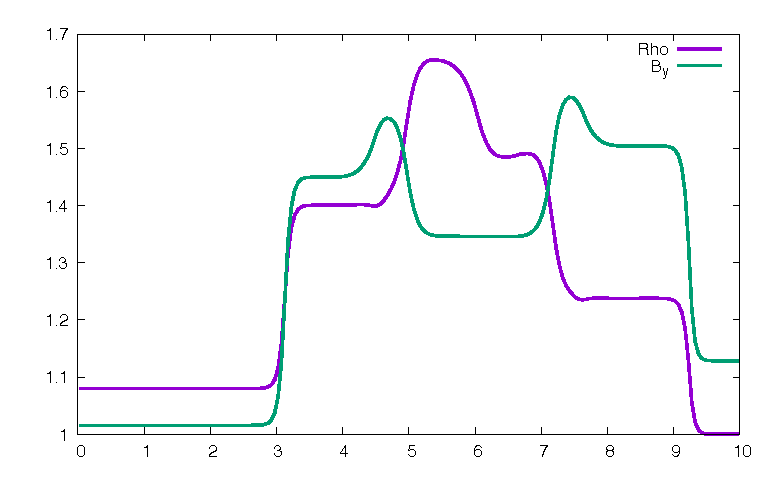
\includegraphics[width=\textwidth]{1D_LLF.eps}
		\end{subfigure}
		\begin{subfigure}{0.75\textwidth}
			\centering
			\caption{Поток HLL.}
			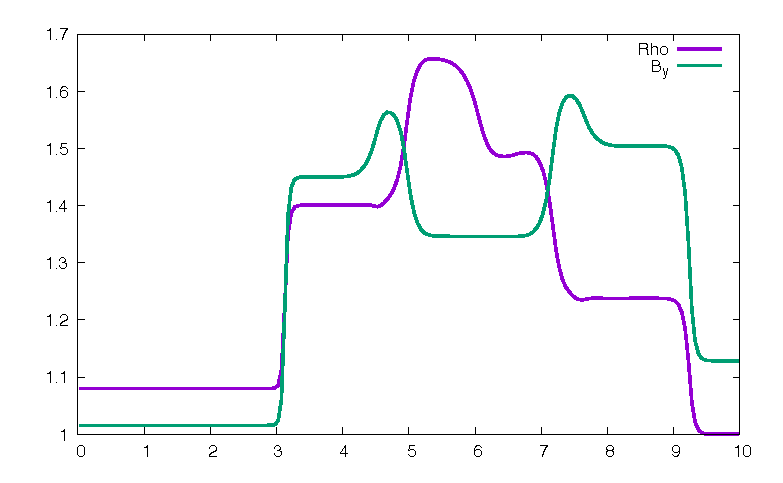
\includegraphics[width=\textwidth]{1D_HLLE.eps}
		\end{subfigure}
	\end{figure}
	\begin{figure}[H]
		\centering
		\caption{$\rho$ и $B_y$ при $t = 1800\tau$.}
		\begin{subfigure}{0.75\textwidth}
			\centering
			\caption{Потоки HLLС.}
			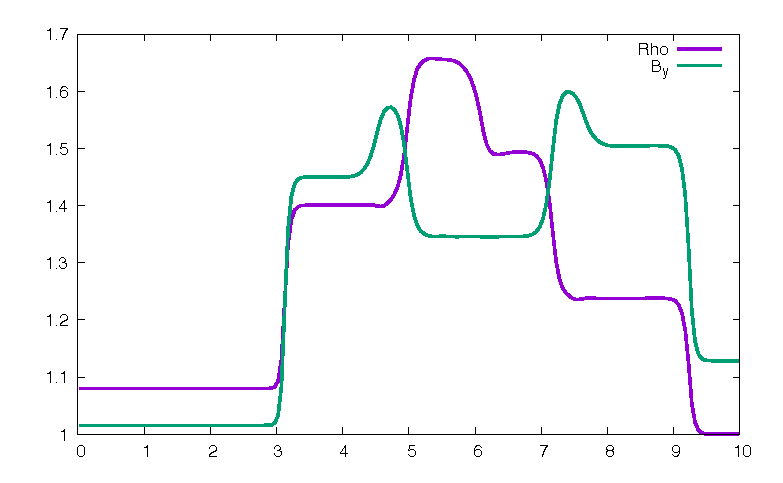
\includegraphics[width=\textwidth]{1D_HLLC.eps}
		\end{subfigure}
		\begin{subfigure}{0.75\textwidth}
			\centering
			\caption{Потоки HLLD.}
			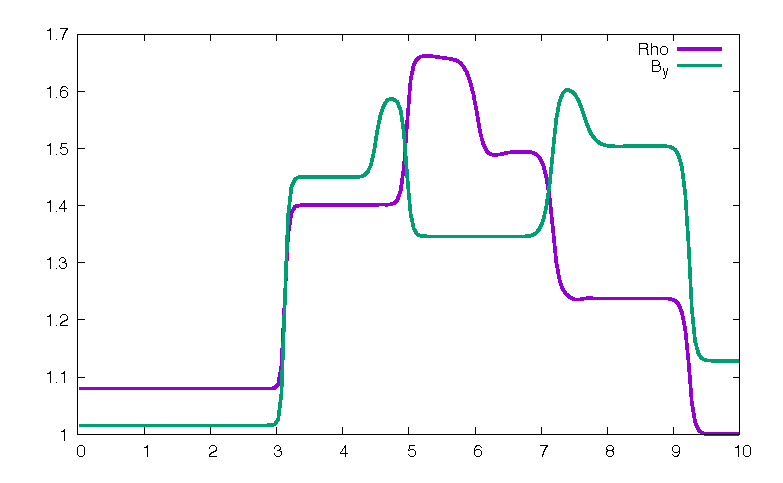
\includegraphics[width=\textwidth]{1D_HLLD.eps}
		\end{subfigure}
	\end{figure}

	%-----------------------------------------------------------------------------
	\subsection{Вихрь Орзака-Тана.}
	%-----------------------------------------------------------------------------

	Вихрь Орзака-Тана (Orszag-Tang Vortex) --
	один из самых распространенных тестов для МГД-системы.
	Областью расчета является единичный квадрат со периодическими 
	граничными условиями на всех сторонах.
	Начальные данные для этого теста задаются так:
	\begin{equation*}
	\begin{split}
		&\rho = \dfrac{25}{36\pi}; p = \dfrac{5}{12\pi}; \gamma = \dfrac{5}{3}; \\
		&v_x = -\sin(2\pi y); v_y = \sin(2\pi x); v_z = 0; \\
		&B_x = -\sin(2\pi y); B_y = \sin(4\pi x); B_z = 0.
	\end{split}
	\end{equation*}
	
	Ниже приведены результаты расчета методом конечных объемов,
	при $\tau = 0.001$ на 256 ячейках по каждому измерению с 
	использованием потоков HLLC.
	
	\begin{figure}[H]
		\centering
		\caption{$\rho$.}
		\begin{subfigure}{0.9\textwidth}
			\centering
			\caption{$t = 2000\tau$}
			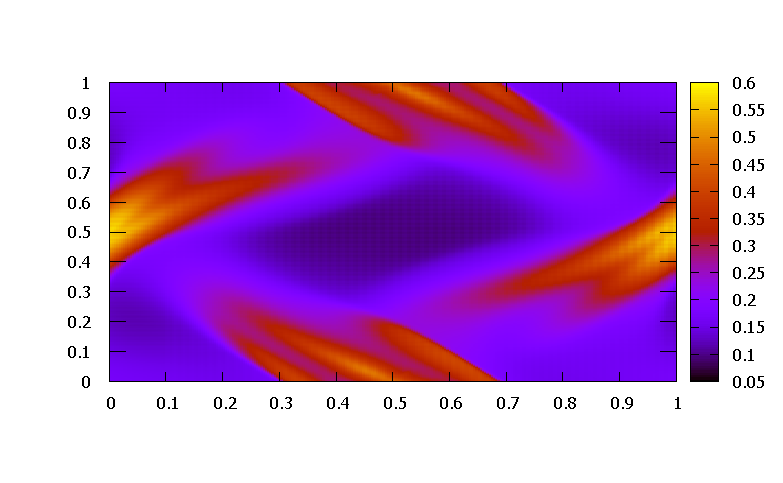
\includegraphics[width=\textwidth]{2D_HLLC_OT_2000.eps}
		\end{subfigure}
		\begin{subfigure}{0.9\textwidth}
			\centering
			\caption{$t = 4000\tau$}
			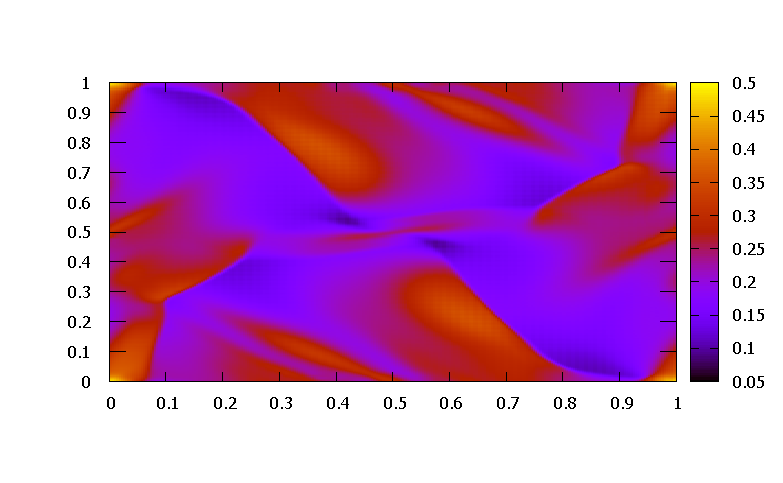
\includegraphics[width=\textwidth]{2D_HLLC_OT_4000.eps}
		\end{subfigure}
	\end{figure}

	\begin{figure}[H]
		\centering
		\caption{$\rho$.}
		\begin{subfigure}{0.9\textwidth}
			\centering
			\caption{$t = 10000\tau$}
			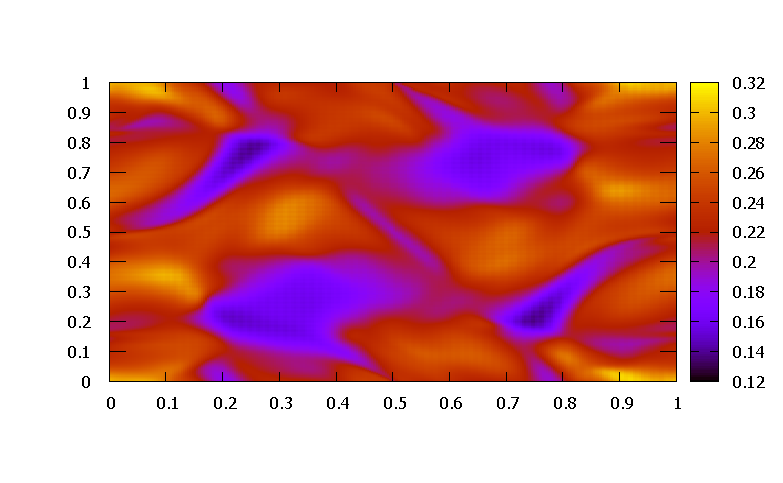
\includegraphics[width=\textwidth]{2D_HLLC_OT_10000.eps}
		\end{subfigure}
		\begin{subfigure}{0.9\textwidth}
			\centering
			\caption{$t = 20000\tau$}
			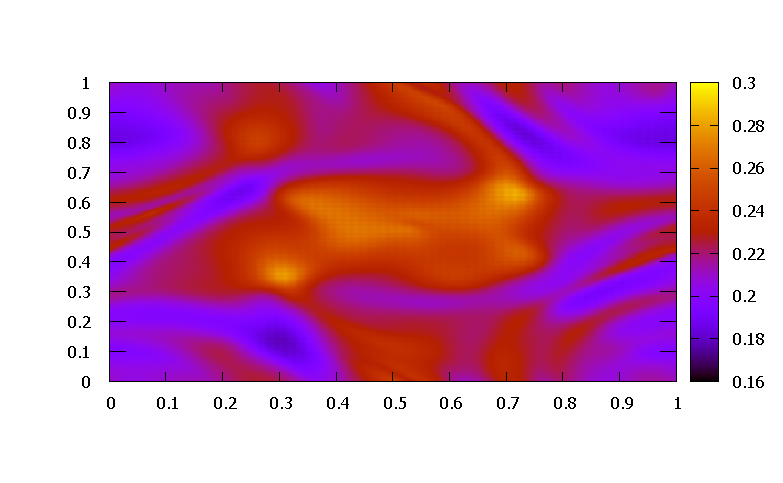
\includegraphics[width=\textwidth]{2D_HLLC_OT_20000.eps}
		\end{subfigure}
	\end{figure}
	
	%%%%%%%%%%%%%%%%%%%%%%%%%%%%%%%%%%%%%%%%%%%%%%%%%%%%%%%%%%%%%%%%%%%%%%%%%%%%%%
	%%%%%%%%%%%%%%%%%%%%%%%%%%%%%%%%%%%%%%%%%%%%%%%%%%%%%%%%%%%%%%%%%%%%%%%%%%%%%%
	\chapter*{Заключение}
	%%%%%%%%%%%%%%%%%%%%%%%%%%%%%%%%%%%%%%%%%%%%%%%%%%%%%%%%%%%%%%%%%%%%%%%%%%%%%%
	%%%%%%%%%%%%%%%%%%%%%%%%%%%%%%%%%%%%%%%%%%%%%%%%%%%%%%%%%%%%%%%%%%%%%%%%%%%%%%
	\addcontentsline{toc}{chapter}{Заключение} 
	
	В ходе работы были рассмотрены получение и свойства системы уравнений магнитной 
	гидродинамики, построены конечно-объемные схемы Годуновского типа
	и схемы разрывного метода Галеркина повышенного порядка аппроксимации
	для неструктурированных сеток, проведены тестовые расчеты
	одномерных в двумерных задач.
	
	Качественно лучшие результаты для задачи о распаде разрыва
	были получены применением разрывного метода Галеркина 
	с использованием потоков HLLD,
	а для вихря Орзака-Тана -- с использованием потока HLLC, который
	зарекомендовал себя как наиболее устойчивый при хорошей 
	разрешающей способности для многомерных задач.
	
	Исходный код реализации построенных методов
	доступен по адресу \url{https://github.com/Jhuighuy/OrchidSolver}
	
	
	\clearpage
	
	
	
	
	
	%%%%%%%%%%%%%%%%%%%%%%%%%%%%%%%%%%%%%%%%%%%%%%%%%%%%%%%%%%%%%%%%%%%%%%%%%%%%%%
	%%%%%%%%%%%%%%%%%%%%%%%%%%%%%%%%%%%%%%%%%%%%%%%%%%%%%%%%%%%%%%%%%%%%%%%%%%%%%%
	%\chapter*{Литература}
	%%%%%%%%%%%%%%%%%%%%%%%%%%%%%%%%%%%%%%%%%%%%%%%%%%%%%%%%%%%%%%%%%%%%%%%%%%%%%%
	%%%%%%%%%%%%%%%%%%%%%%%%%%%%%%%%%%%%%%%%%%%%%%%%%%%%%%%%%%%%%%%%%%%%%%%%%%%%%%
	\addcontentsline{toc}{chapter}{Литература} 
	\bibliographystyle{utf8gost705u}
	\bibliography{Biblio}
	
\end{document}
